\begin{minipage}[t][\PosterTopRowHeight][t]{\PosterTwoWidth}\vspace{0pt}
  \begin{TicketTwoPanel}{\PosterTopRowHeight}{2}{WHAT WE FOUND: TWO SAFE RETUNES, ONE UNSAFE GRID}

    {\FigureSize Buses 30 and 37 each replace a little more SG ($\rho:0.875\to0.885$, $+7.9$ MW GFL in total). At each site we adjust the gains so that the shared 4.9 Hz mode keeps its decay rate, $0.0657\ \mathrm{s^{-1}}$.\par}
    \vspace{3mm}
    \noindent\begin{minipage}[c]{282mm}\centering
      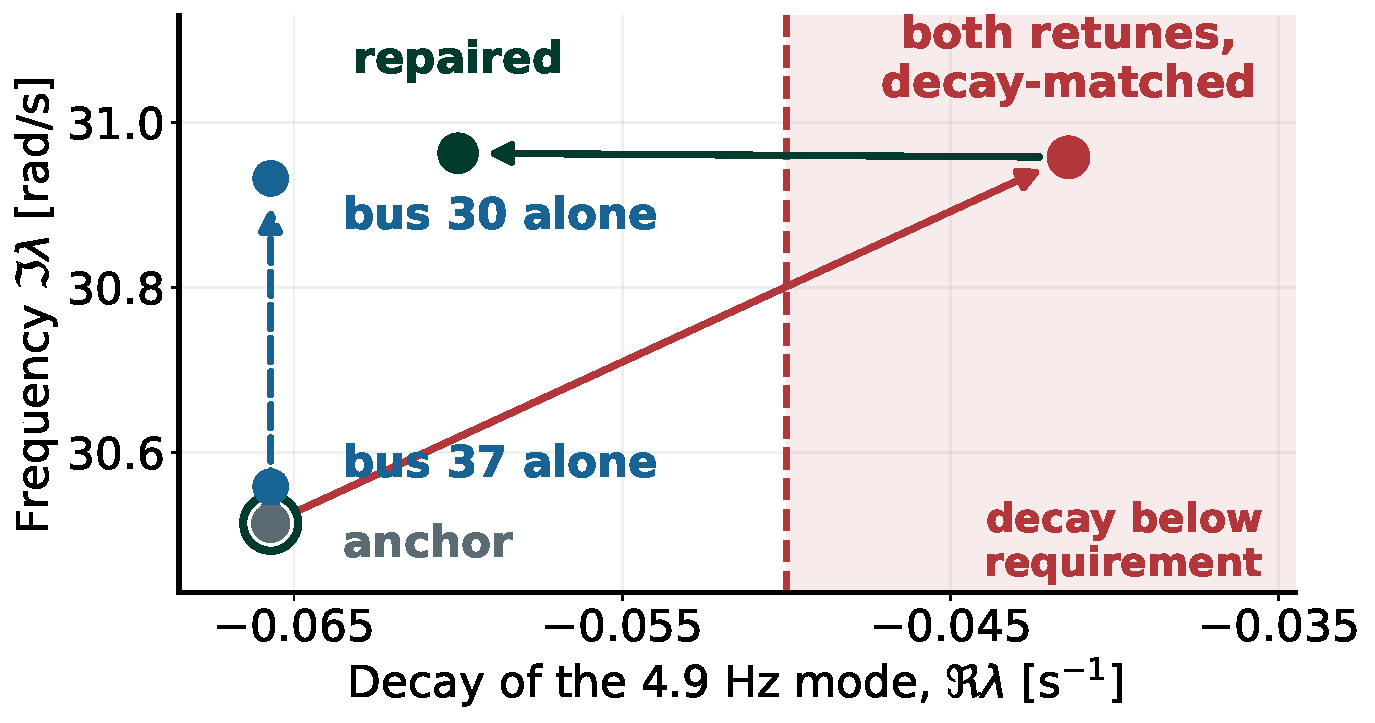
\includegraphics[width=280mm,height=132mm,keepaspectratio]{generated/figures/splane.pdf}
    \end{minipage}\hfill%
    \begin{minipage}[c]{112mm}\raggedright
      {\PosterCondensed\bfseries\fontsize{60pt}{64pt}\selectfont\color{IASVermillion}$0.0243$\par}
      {\FigureSize s$^{-1}$ of decay lost to the interaction (certified $\pm4\times10^{-7}$)\par}\vspace{4mm}
      {\MetricSize\bfseries\color{IASDarkGreen}87.6\,\%\par}
      {\FigureSize GFL share after the repair: 4,735 MW inverter, 667 MW SG kept\par}
    \end{minipage}\par
    \vspace{3mm}
    {\EquationSize\color{IASBlue}$\mathcal I=\Re\lambda_{\text{both}}-\Re\lambda_{30}-\Re\lambda_{37}+\Re\lambda_{\text{anchor}}=+0.0243\ \mathrm{s^{-1}}$\par}
    \vspace{3mm}
    \begin{InWords}\InWordsLabel Each site fixes the decay as if the other were not changing, and the two fixes do not add up: together the decay falls to $0.0414$, below the $0.05$ required. The mode is still stable; only its margin is lost. Matching the whole pole instead (decay and frequency) at each site keeps it at $0.0657$.\end{InWords}

  \end{TicketTwoPanel}
\end{minipage}%
